\chapter{Introdução}





\section{Objetivos}

Neste projeto iremos propor e avaliar a eficácia da utilização de um modelo para estimar o comportamento dos juros da dívida técnica. Conforme descrito na seção \ref{elementos_td}, os juros são todo o esforço adicional necessário para realizar as atividades de desenvolvimento de um software. Esse esforço adicional é causado pela existência de uma dívida técnica. Neste trabalho, iremos estimar o quanto de juros é criado para um determinado tipo de dívida técnica. Digamos que o esforço necessário para realizar uma modificação em uma classe $\textbf{y}$ seja igual à $\textbf{w}$ em um cenário onde não exista um determinado tipo de dívida técnica $\textbf{z}$ na classe $\textbf{y}$. Caso a dívida técnica $\textbf{z}$ existisse na classe $\textbf{y}$ o esforço necessário para realizar a modificação seria igual a $\bar{\overline{\textbf{w}}  = \textbf{xw}}$  onde $\textbf{x}$  é o fator de acréscimo  de esforço causado pela dívida técnica.  Pouco se sabe a respeito de como o valor de $\textbf{x}$  varia para cada tipo de dívida técnica e qual o seu comportamento com o passar do tempo. Neste trabalho pretendemos fornecer um modelo para ajudar na compreensão do comportamento de $\textbf{x}$ ao:

\begin{enumerate}
\item Indicar o valor relativo de $\textbf{x}$ em relação aos tipos de dívida técnica considerados na pesquisa. Ou seja, estabeleceremos uma relação de ordem para o conjunto de tipos de dívidas técnicas que iremos analisar. Essa relação de ordem irá definir quais tipos de dívida técnica, dentre os analisados, apresentam maiores juros.
\item Indicar como o valor de $\textbf{x}$ varia durante o desenvolvimento do projeto de software. 

\end{enumerate}



\section{Questões de Pesquisa}

Especificamente, pretendemos responder as seguintes questões de pesquisa:

\subsubsection{QP1: Dentre as ocorrências de dívida técnica de design e código que serão analisadas, quais produzem maior juros?}

Obter uma estimativa para os juros dos tipos de dívida técnica analisados nesta pesquisa permitirá um aprimoramento no gerenciamento da dívida técnica. Uma das vantagens é que a priorização poderá ser simplificada.  A escolha de quais dívidas deverão ser priorizadas poderá ser feita de forma mais objetiva. Apesar de ser possível remover a objetividade ao utilizar dinâmicas de estimação como a técnica Delphi\cite{hsu2007delphi} e o Planning Poker\cite{haugen2006empirical} para a elaboração de estimativas dos juros da dívida técnica, essas técnicas exigem o envolvimento de especialistas no software e pode levar tempo para que se chegue em um consenso. Seria mais vantajoso se esse processo de estimação dos juros pudesse ser realizado de forma mais automática ou ao menos sem exigir tanto envolvimento de pessoas e ainda sim apresentar um grau de acurácia adequado. A priorização do pagamento da dívida técnica torna-se simples caso estejam a disposição estimativas precisas a respeito do principal e do juros. Uma exemplo de estratégia para a priorização poderá ser analisar a razão entre os os juros e o principal . Quanto maior o resultado, maior deve ser a prioridade de pagamento da dívida. 

Ao respondermos a questão de pesquisa 1 (QP1), indiretamente forneceremos auxílio para que as seguintes questões possam ser respondidas: 

\begin{itemize}
\item Quais dívidas técnicas devem ser terminantemente evitadas?
\item Quais dívidas devem ter seu pagamento priorizado?


\end{itemize}

\subsubsection{QP2: O acúmulo de juros em relação ao tempo é linear ou composto?}

O comportamento do juros de uma dívida técnica no decorrer dos ciclos de desenvolvimento e manutenção do software tem um papel importante no gerenciamento. O entendimento a respeito de como acontece o crescimento dos juros com o passar do tempo também pode ser incorporado as atividades de priorização no gerenciamento da dívida técnica.

\section{Limitação do escopo}

Para tornar o projeto viável, em função do tempo e tecnologias disponíveis para realizá-lo, iremos restringir nossa análise a dívidas técnicas de design, código e testes. Apesar de existirem diversos tipos de dívida técnica, conforme mostrado na seção \ref{sec:tipos_td}, muitos desses tipos são pouco tangíveis ou quantificáveis, tais como as dívidas técnicas de processo e tecnologia. Logo, há uma dificuldade para serem analisados automaticamente, como pretendemos fazer neste trabalho. Dessa forma, iremos restringir esta pesquisa a tipos de dívida técnica que possam ser observadas no código do software.  Além disso,  iremos apenas nos dedicar a projetos escritos na linguagem Java. Os tipos de dívida técnica que iremos estudar nesta pesquisa estão apresentados na tabela \ref{table:tiposDivida}, onde as dívidas são divididas em tipo e subtipo. Os tipos utilizados são os descritos na seção \ref{sec:tipos_td} e separam as dívidas em grupos mais gerais. Os subtipos são ocorrências específicas de dívida técnica de um tipo.  Novos tipos e subtipos poderão ser acrescentados ou removidos da tabela \ref{table:tiposDivida} durante a pesquisa. Uma nova dívida técnica será acrescentada caso a operacionalização de sua detecção seja possível de ser realizada dentro do tempo disponível para a pesquisa. 


\begin{table}[]
\centering
\caption{Dívidas técnicas que serão analisadas neste trabalho.}
\label{table:tiposDivida}
\begin{tabular}{|l|l|}
\hline
\bf{Tipo}   & \bf{Subtipo}                            \\ \hline
Código & Código duplicado                   \\ \hline
Design & \textit{God Class}\cite{fowler2009refactoring}                          \\\hline
Testes & Ausência de testes unitários       \\\hline
Design & Complexidade ciclomática excessiva \\\hline
Código       & Método com muitos parâmetros                                    \\\hline
Código       & Método muito extenso                                    \\\hline
Design       & \textit{Feature envy}\cite{fowler2009refactoring}                                   \\\hline
Design       & \textit{Lazy Class}     \cite{fowler2009refactoring}    \\\hline                         
\end{tabular}
\end{table}

\section{Conclusões}

A escolha dos nossos objetivos foi feita com o intuito de diminuir o nível de subjetividade durante a realização das atividades relacionadas ao gerenciamento dos juros da dívida técnica. Em vez de opiniões formadas por experiências individuais, sugerimos a utilização de dados empiricamente obtidos  para aumentar o nível de segurança das decisões que serão realizadas em relação aos juros da dívida técnica. Particularmente, desejamos auxilizar as atividades de priorização do pagamento.  Esse auxílio será dado ao fornecermos um modelo de estimação dos juros. Esse elemento é um fator importante para a tomada de decisões, pois os juros são o que realmente fazem com que exista a necessidade de que a dívida técnica seja gerenciada. Caso, não houvesse nenhuma consequência ao se adquirir uma dívida técnica, não haveria necessidade de gerenciá-la. Os juros são as consequências de se inserir dívidas técnicas em um software.






DESCREVER IMAGEM CITACOE e CORRIGIR GRAFICO.

  \begin{figure}[H]
  \centering
  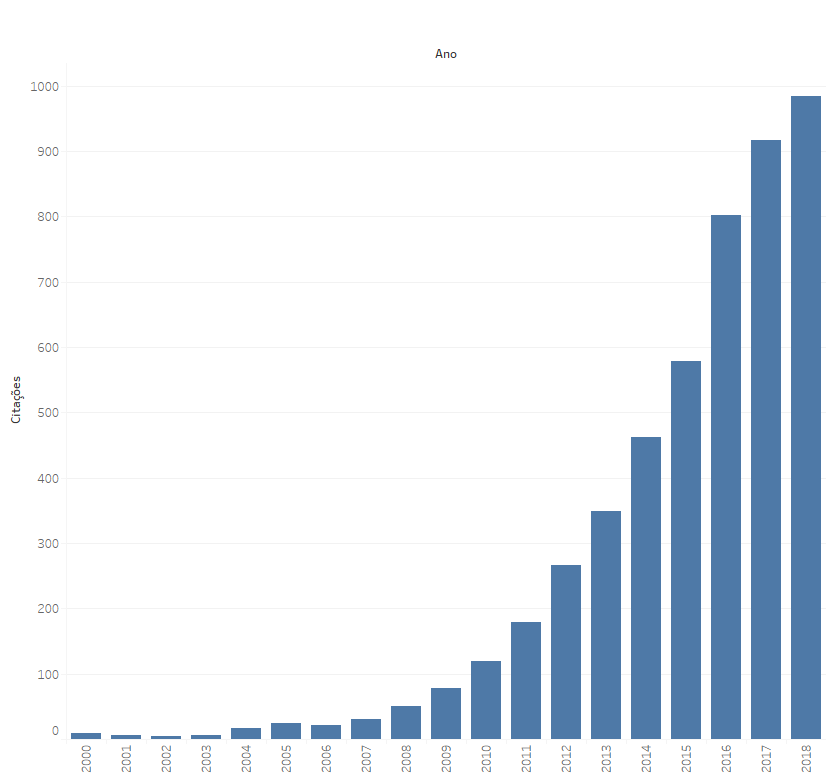
\includegraphics[width=15.28cm,height=10.65cm]{introducao/CitacoesDividaTecnica.png} 
  \caption{Número anual de citações ao termo dívida técnica. }
  \label{fig:cap1_citacoes_td_ano} 
\end{figure}

Um dos papéis da engenharia de software é fornecer métodos, modelos e técnicas para que o software atenda às necessidades dos interessados em sua construção. A utilização desse conhecimento leva a uma forma aproximadamente ideal de realizar as atividades necessárias para o desenvolvimento do software. Os resultados  gerados por atividades feitas dessa forma apresentarão um elevado grau de qualidade. Entretanto, essa forma ideal de realizar as atividades pode exigir recursos incompatíveis com os disponíveis para o projeto. Por este motivo, as pessoas envolvidas com o projeto do software tendem a realizar essas atividades de forma que atendam às restrições de recursos e, ainda assim, estejam o mais próximas possíveis da forma ideal. Entretanto, a existência de restrições de recursos demasiadamente severas fazem com que algumas atividades tenham de ser realizadas de uma forma muito distante da ideal. Os resultados produzidos pelas atividades feitas de tal forma são chamados de dívida técnica. O nome em questão foi dado a esse fenômeno  devido as suas semelhanças com a dívida financeira. Realizar uma atividade de forma não ideal é como adquirir uma dívida para com a qualidade do sistema. Uma característica da dívida técnica é a de que enquanto ela não for paga, ou seja, enquanto a atividade não seja refeita produzindo resultados mais próximos do ideal, haverá um esforço adicional para realizar futuras atividades relacionadas a dívida técnica. Esse esforço adicional é equivalente ao juros financeiros que devem ser pagos enquanto o valor emprestado não for devolvido.  


%O que é dívida técnica
A dívida técnica é uma metáfora para um tipo de degradação que ocorre no software com o passar do tempo. Essa degradação é a consequência de se realizar, sem um nível de qualidade satisfatório, as atividades necessárias para o desenvolvimento do software. Essas atividades são realizadas de forma inadequada por diversas razões. Seja por falta de conhecimento, descuido ou devido a restrições de recursos. Um exemplo em que normalmente são criadas dívidas técnicas é quando o prazo definido para realizar uma determinada atividade não é compatível com a complexidade e o esforço necessário para completá-la de forma adequada. Dessa forma, para evitar a perda do prazo e suas eventuais consequências, opta-se por realizar as atividades de desenvolvimento sem um nível de qualidade satisfatório, porém atendendo as necessidades do produto. Há ainda casos onde as dívidas técnicas são criadas apenas pela passagem do tempo. Isso acontece quando uma tecnologia utilizada se torna obsoleta e não é substituida e fica cada vez  mais difícil lidar com os artefatos criados com essa tecnologia. Isso acontece pela diminuição do número de profissionais que dominam essa tecnologia obsoleta como também pelas mudanças de paradigmas observadas comparando as tecnologias atuais e as obsoletas presentes nos software. Apesar da metáfora propiciar uma forma padrão de comunicar esse fenômeno, a  dívida técnica pode ser entendida como tudo aquilo no software que não é necessário, mas faz com que seja mais difícil evoluí-lo.

O termo dívida técnica foi usado pela primeira vez por Cunningham\cite{cunningham1993wycash}. Ele percebeu que criar porções de código, que não estivessem de acordo com as boas práticas da programação orientada a objetos, podia trazer maior velocidade para o desenvolvimento do software, desde que esse código fosse reescrito brevemente de forma correta. A inserção dessas porções de códigos inapropriados é semelhante a contrair uma dívida para com  o sistema e todo esforço adicional necessário para evoluir as porções de código feitas dessa forma são os juros dessa dívida. Inicialmente, a dívida técnica foi associada apenas à degradação do código do software. Porém, à medida que esse fenômeno foi melhor compreendido, ele foi identificado também em outros elementos do software como testes, arquitetura, documentação e processo. 


O gerenciamento da dívida técnica consiste na aplicação de estratégias para mantê-la em patamares aceitáveis. Negligenciar esse gerenciamento pode trazer consequências negativas para os projetos de desenvolvimento de software. Caso a dívida técnica atinja um patamar muito alto, é possível que todo o processo de desenvolvimento e evolução do software fique inviabilizado. Esta inviabilidade se concretiza quando o esforço necessário para inserir novas funcionalidades é maior do que os benefícios ao produto trazidos por elas.




\section{Motivação}
EVIDENCIAR ENFASE EMPIRICA DO TRABALHO.

Os malefícios da dívida técnica foram estudados e documentados na literatura\cite{zazworka2011investigating,power2013understanding}. Um deles está relacionado à produtividade das equipes responsáveis pelo software. À medida que a dívida técnica é acumulada inadvertidamente, ocorre uma variação negativa na produtividade.  Cada vez mais atividades são realizadas apenas para estabilizar o software em vez de adicionar funcionalidades e melhorias. Em certos casos, inclusive, é cogitado o descarte do software atual a fim de que uma nova versão seja produzida do início \cite{sterling2010managing}. Uma das dificuldades para a realização do gerenciamento da dívida técnica é a falta de técnicas que auxiliem a execução dessa atividade. A inexistência dessas técnicas padronizadas é causada pelo fato de que grande parte do conhecimento que existe a respeito da dívida técnica foi gerado por experiências individuais e contextuais. Dessa forma, esse conhecimento não foi devidamente validado por meio de evidências empíricas. Isso faz com que as técnicas de gerenciamento  da dívida técnica sejam escassas e não confiáveis\cite{brown2010managing}. 

Basicamente, para que o gerenciamento da dívida técnica possa ser realizado é necessário estimar duas informações:
(i)	O esforço necessário para corrigir uma dívida técnica. Essa informação é denominada como o \textbf{principal} da dívida técnica.
(ii)	O esforço adicional necessário para realizar as futuras atividades de desenvolvimento, evolução e manutenção do software.  Esse esforço adicional é chamado de \textbf{juros} da dívida técnica. Existe uma necessidade especial em gerenciar os juros da dívida técnica. Isso acontece pois os juros são aquilo que efetivamente influenciam negativamente os projetos de software.  Obter estimativas a respeito dos juros é uma das principais atividades do gerenciamento da dívida técnica. O principal em si, ou seja, o esforço necessário para quitar uma dívida técnica não traz nenhuma dificuldade adicional para o projeto de software. O que faz com que seja necessário alocar recursos para quitar uma dívida técnica é o quanto os juros dessa dívida estão altos. Além da escassez de estudos sobre o cálculo dos juros da dívida técnica, existe uma falta ainda maior de trabalhos empíricos ou que tenham sido validados de alguma forma. 

\section{Trabalhos relacionados aos juros da dívida técnica}
\label{modelos_existentes}

Por se tratar de um aspecto importante no gerenciamento da dívida técnica, a estimação e modelagem dos juros foram abordadas em alguns trabalhos encontrados na literatura. Foram propostos modelos e ferramentas para calcular os juros da dívida técnica. Entretanto, essas abordagens focaram em uma medida geral para os juros da dívida em todo o software. Não encontramos trabalhos focados em medir os juros relativos a instâncias de tipos específicos de dívida técnica. Logo, não encontramos uma abordagem que tenha como foco a medição dos juros decorrentes da existência de um determinado tipo de dívida técnica. A seguir descreveremos alguns desses trabalhos.

Foram encontrados alguns trabalhos que também propõem algum modelo para estimação ou gerenciamento dos juros da dívida técnica. Nesse trabalho \cite{singh2014framework}, Singh et al. propõem um arcabouço para estimação dos juros da dívida técnica. Esse arcabouço combina métricas de manutibilidade com informações 
sobre a compreensão do código. As métricas de manutibilidade são extraídas usando técnicas descritas na literatura.  Enquanto isso, as informações sobre 
compreensão são obtidas por meio de uma ferramenta desenvolvida pelos autores. Essa ferramenta é inserida em um ambiente integrado 
de desenvolvimento (IDE) e monitora a interação dos desenvolvedores com o código do software. Esse monitoramento armazena informações tais como quantas vezes uma mesma classe foi
acessada em um determinado intervalo de tempo e quanto tempo uma classe ficou aberta no editor. Os autores acreditam que as métricas de manutibilidade indicam a 
existência de dívida técnica em uma classe enquanto que as informações sobre compreensão podem ser usadas para estimar o quanto de juros essas dívidas estão 
gerando. A estimativa de juros é feita calculando a diferença do nível de compreensão em classes onde existe e classes onde não existe dívida técnica.

Em \cite{nugroho2011empirical} Nugroho et al. sugerem um modelo para calcular o principal e os juros da dívida técnica. Para tal, é utilizado um método de avaliação de qualidade
previamente definido pelos autores. Esse método classifica os sistemas em cinco categorias. Quando um sistema está na categoria mais alta, ele apresenta um elevado grau
de qualidade. Por outro lado, quando um sistema está na categoria mais baixa ele apresenta muitos problemas de qualidade. Essa qualidade é medida utilizando métricas
de acoplamento e coesão já definidas na literatura. Os autores usam um conjunto de 44 sistemas para obter dados e estimar a quantidade média de linhas que
 devem ser alteradas para levar um sistema de uma categoria para outra, superior. O principal da dívida técnica de um sistema é estimado pela quantidade de linhas necessárias
 para levar o sistema de seu nível atual de qualidade para o nível de maior qualidade. Enquanto isso, os juros são estimados como a diferença entre o esforço necessário para evoluir o software no nível atual e o esforço que seria necessário caso o software estivesse no nível mais alto de qualidade. 
 
 Uma das características que podemos observar nesses modelos de estimação dos juros é a de que eles têm como objetivo estimar a quantidade total de juros de um sistema. Esse objetivo é útil quando o foco é monitorar a dívida técnica de modo que ela não atinja patamares muito altos e inviabilize o continuidade do projeto. Entretanto, essas medidas gerais não auxiliam a priorização do pagamento da dívida técnica. A priorização consiste em selecionar, dentre as dívidas técnicas existentes em um software, quais devem ser pagas mais rapidamente. Essa escolha envolve principalmente a avaliação dos efeitos negativos que essas dívidas trazem para o projeto. Ou seja, a priorização do pagamento considera quais dívidas gerarão maiores juros. Neste trabalho, o modelo de estimação proposto tem como objetivos avaliar os juros para tipos ou instâncias específicas de dívidas técnicas. Com isso, acreditamos complementar os trabalhos já existentes e avançar o estado da arte do gerenciamento dos juros da dívida técnica. 



\section{Contribuições}

Neste trabalho iremos propor  um modelo para estimar os juros gerados pelas dívida técnicas. Diferentemente dos modelos descritos na seção \ref{modelos_existentes}, o objetivo a ser alcançado com esse modelo é identificar quais tipos de dívida técnica apresentam mais juros e ,dessa forma, precisam ser evitados. Esse modelo utilizará dados extraídos de repositórios públicos de software. Diversos projetos serão analisados utilizando técnicas de mineração de repositórios e inferência estatística. 

Com a aplicação do modelo que proporemos, pretendemos responder às seguintes questões de pesquisa:

\begin{itemize}
\item QP1: Dentre as ocorrências de dívida técnica de design e código que serão analisadas, quais produzem maior juros?
\item QP2: O acúmulo de juros em relação ao tempo é linear ou composto?
\end{itemize}



\section{Organização do texto}

O restante deste texto é organizado da seguinte forma. No capítulo 2 descrevemos a dívida técnica. São apresentadas as formas de classificação encontradas na literatura e os diversos tipos de dívida técnica. No capítulo 3 fornecemos um panorama a respeito da pesquisa  sobre a dívida técnica. No capítulo 4 descrevemos os objetivos deste trabalho e quais questões de pesquisa serão respondidas. No capítulo 5 definimos a metodologia que será aplicada juntamente com o cronograma. Por fim, fornecemos as referências bibliográficas que utilizamos para a realização desta pesquisa.


